% \documentclass[12pt,openright,oneside,a4paper,brazil]{abntex2}
% \usepackage[utf8]{inputenc}
% \counterwithout{section}{section}
% \counterwithout{figure}{chapter}
% \counterwithout{table}{chapter}
% \setlength{\parindent}{1.3cm}
% \usepackage{indentfirst}
% \setlength{\parskip}{0.2cm}
% \usepackage[bottom=2cm,top=3cm,left=3cm,right=2cm]{geometry}
% \usepackage{graphicx}
% \graphicspath{{figuras/}}
% \usepackage{placeins}
% 
% %opening
% \title{}
% \author{}
% 
% \begin{document}
% 
% 
% \textual
\begin{center}
 {\large Plano de gerenciamento de Qualidade}\\[0.2cm]
 {Planta de abastecimento de água potável a partir da umidade do ar}\\
 \end{center}
 
 \section*{Histórico de Alterações}
\begin{table}[h]
\centering
\begin{tabular}{|c|c|p{6cm}|p{5cm}|}
Data & Versão & Descrição & Responsável\\
\hline                               
22/04/2015 & 0.0 & Criação do plano de gerenciamento de qualidade & Alexandre Kryonidis, André Luís, Matheus Jericó\\
\hline
\end{tabular}
\end{table}

\section*{Objetivo}
	O objetivo desse plano é estabelecer um processo de gerenciamento e controle da qualidade do projeto.
        
\section*{Descrição dos processos de gerenciamento da qualidade}
	A qualidade de um projeto está relacionada, principalmente, com o cumprimento dos requisitos levantados, ou seja, satisfaz os objetivos a que o projeto se propôs a solucionar. Dessa forma pretende-se gerenciar a qualidade do projeto da seguinte maneira:
\begin{itemize}
\item As alterações nos requisitos de qualidade previstos para o sistema devem passar por uma avaliação do sistema de controle de mudanças da qualidade.
\item Todas as reclamações provenientes dos "stakeholders" serão avaliadas e, ao corrigi-las, deverão ser tratadas como medidas corretivas no plano de gerenciamento da qualidade.
\item Todos os produtos ou entregas que não cumprem obedecem a declaração de escopo deverão ser tratadas como medidas corretivas no plano de gerenciamento de qualidade.
\item As solicitações de mudanças devem ser documentadas de acordo com o plano de comunicações do projeto.
\end{itemize}

\section*{Priorização das mudanças nos quesitos de qualidade e respostas}
\begin{itemize}
\item  \textbf{Prioridade Alta}

	Mudanças de alta prioridade causam um grande impacto no projeto e deverão ser tratadas em caráter de urgência pelo gerente do projeto e, se possível, em conjunto com algum membro da equipe de qualidade. Apesar de o gerente do projeto ter autonomia de fazer as modificações necessárias, essas mudanças deverão ser mencionadas durante as reuniões de grupos devido a sua relevância. 
        
        
\item  \textbf{Prioridade Média}

	Mudanças de média prioridade envolvem um impacto que requer ação rápida do Gerente de Projeto, de preferência em conjunto com integrantes da equipe de qualidade. Decisões podem ser feitas antes das reuniões de controle, mas também é possível esperar um pequeno prazo para serem avaliadas por um número maior de “steakholders”. Os resultados dessa mudança também devem ser mencionados nas reuniões.
        
\item  \textbf{Prioridade Baixa}

	Mudanças de prioridade Baixa não acarretam alterações significativas na elaboração do projeto e, portanto, não é requerida uma ação imediata, está dentro da autonomia de qualquer integrante da gerência do Projeto.
\end{itemize}

\section*{Sistema de controle de mudanças da qualidade}
	As mudanças relacionadas a qualidade do projeto devem ser tratadas segundo o fluxo apresentado a seguir. As conclusões de maior importância devem ser apresentadas nas reuniões de controle.
   \begin{figure}[!h]
    \centering
    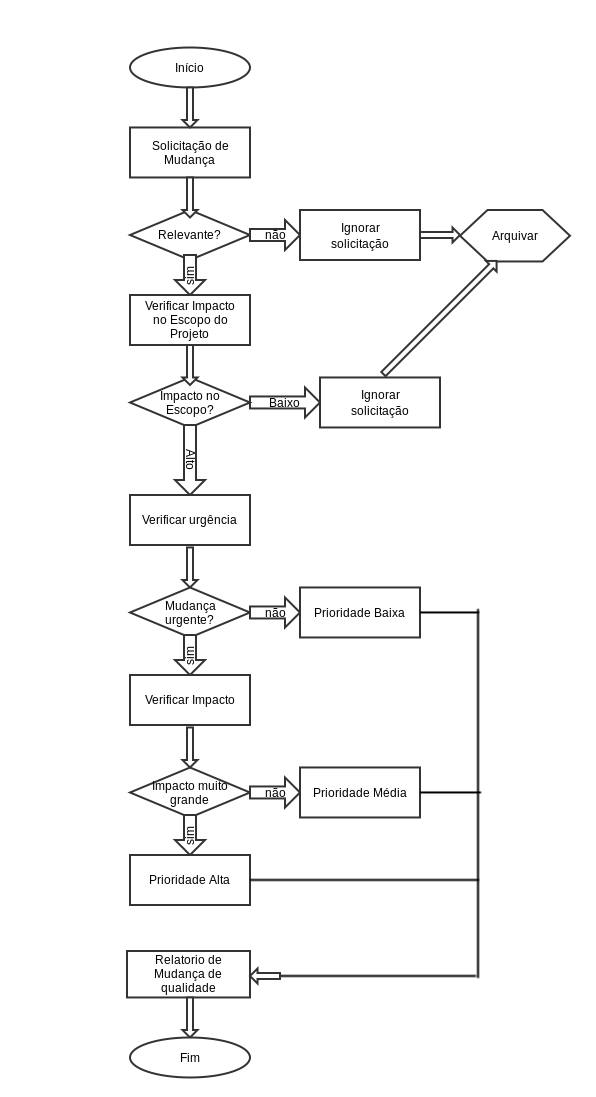
\includegraphics[scale = 0.6]{editaveis/figuras/fluxo_qualidade}
    \label{fluxo_qualidade}
    \caption{Fluxo do controle de mudanças da qualidade}
   \end{figure}
   \FloatBarrier
   
   
\section*{Frequência de avaliação dos requisitos de qualidade do projeto}
	Os requisitos de qualidade serão avaliados e, caso necessário, atualizados de duas em duas semanas. Os resultados obtidos a partir das análises relacionados a qualidade do projeto serão apresentados nas reuniões presenciais do grupo.
             
\section*{Alocação financeira das mudanças nos requisitos de qualidade}
        Todas as mudanças a serem efetuadas devem estar dentro do previsto pela equipe de gerenciamento de custos, qualquer outra alteração que cause um impacto significativo no orçamento do projeto deverá ser debatido em conjunto com o gerente de custos e o gerente de projeto. Como, a princípio, esse projeto não é patrocinado, é difícil adquirir recursos adicionais, por isso, gastos extras devem ser evitados. Caso o gasto adicional traga benefícios consideráveis para o projeto, ele não deverá ser descartado. Qualquer necessidade de avaliação de custos será atribuída a equipe de gerenciamento de custo, ou será enviado a eles um relatório que estará sujeita a análise e aprovação.
        
\section*{Administração do plano de gerenciamento da qualidade}

\begin{enumerate}
\item Responsável pelo plano:
\begin{itemize}
\item Alexandre Torres Kryonidis
\item Andre Luís Motoshima Barros
\end{itemize}
\item 2. Frequência de atualização do plano de gerenciamento da qualidade

	O plano de qualidade será avaliado quinzenalmente e será atualizado, caso necessário, após essas avaliações. Qualquer necessidade de alteração no plano antes desse período, deverá ser tratado segundo os procedimentos tratados pelo tópico \textit{Outros assuntos relacionados ao gerenciamento da qualidade do projeto não previstos neste plano}.
\end{enumerate}

\section*{Outros assuntos relacionados ao gerenciamento da qualidade do projeto não previstos nesse plano}
	Qualquer solicitação que não se enquadre nos preceitos deste plano deverá ser abordada nas reuniões semanais de acompanhamento do projeto, dessa forma, será dado o devido encaminhamento. Após as aprovações, o plano de gerenciamento será atualizado com os devidos registros.

\section*{Assinaturas}
\begin{center}
Data: \rule{0.5cm}{0.1mm}/\rule{0.5cm}{0.1mm}/\rule{1cm}{0.1mm}     \\
\rule{13cm}{0.1mm}\\
ADRIANNY VIANA DE ARAÚJO AMORIM – GERENTE DE PROJETO\\
\rule{13cm}{0.1mm}\\
ALEXANDRE TORRES KRYONIDIS- GERENTE DE QUALIDADE
\end{center}
% \end{document}